\documentclass[preprint,12pt]{elsarticle}
\usepackage[utf8]{inputenc}
\usepackage{amsmath}
\usepackage{graphicx}
\usepackage{booktabs}
\usepackage{xcolor}
\usepackage[hidelinks]{hyperref}
\usepackage{url}
\newcommand{\repourl}{https://github.com/imanejerrari-etu-bit/iaha-replication-modes}  % set once, then run check_release.py
\newcommand{\todo}[1]{\textcolor{red}{[TODO: #1]}}   % remove every \todo before submission
\newcommand{\perf}{\textsc{performance}}
\newcommand{\cons}{\textsc{consistency}}
\newcommand{\avail}{\textsc{availability}}
\newcommand{\econ}{\textsc{economic}}
\journal{Journal of Systems and Software}

\begin{document}
\begin{frontmatter}
\title{What Replication Modes Cost and Protect: A Measurement Study of Containerised PostgreSQL and Its Implications for Adaptive Mode Selection}

\author[lis]{Imane Jerrari\corref{cor1}}
\ead{imane.jerrari-etu@etu.univh2c.ma}
\author[lis]{Ismail Assayad}
\ead{i.assayad@ensem.ac.ma}
\cortext[cor1]{Corresponding author}
\address[lis]{Laboratory of Information Systems (LIS), Faculty of Sciences Ain Chock \& ENSEM, Hassan II University of Casablanca, Casablanca, Morocco}

\begin{abstract}
Adaptive high-availability controllers for containerised databases choose among replication modes with rules or learned models, yet the labels behind those choices are usually written by hand rather than measured. We measure what four replication modes of PostgreSQL cost and protect, on a cluster managed by the CloudNativePG operator on a single-host Kubernetes testbed with emulated inter-node delay. Over three workloads, three delays and five repetitions (150 cells), and a sweep of 2, 8 and 32 clients (90 cells), synchronous replication costs about one network round trip of latency per commit when the primary is not CPU-saturated, and more under saturation; the resulting loss of write throughput at 10\,ms of one-way delay is 81\%, 68\% and 45\% with 2, 8 and 32 clients. When the primary is isolated from the network and then crashes, asynchronous replication lost about 2,000--2,200 acknowledged transactions per second of isolation (12 of 12 runs), roughly in proportion to the write rate, whereas synchronous replication lost none in 18 of 18 runs; a crash without isolation lost none in 10 of 10 runs. Replaying controllers on the measured outcomes under three declared requirement policies, we find that no fixed mode satisfies the requirements in all contexts (11--100\% of steps in violation), that a rule cascade from our earlier work violates them in 13\% to 47\% of steps, and that one context admits no feasible durable mode. All results come from one laptop, emulated delay and nine contexts; we state what they do not show.
\end{abstract}

\begin{keyword}
replication modes \sep PostgreSQL \sep Kubernetes \sep high availability \sep self-adaptive systems \sep measurement study
\end{keyword}
\end{frontmatter}

\section{Introduction}\label{sec:intro}
Databases increasingly run as containers under orchestrators, where a single configuration choice decides how much latency a write pays and how much data a crash can destroy: whether a commit waits for one or more standby servers (synchronous replication) or returns once the primary has the data (asynchronous replication) \cite{pgdocs,abadi2012}. Operators and failover tools treat this choice as configuration fixed at deployment \cite{cnpg,patroni,repmgr,stolon}. A line of work, including our own, proposes to select the mode at run time from operational telemetry \cite{jerrari2026iaha}.

Such a controller is only as good as the evidence behind its decisions. In our earlier studies \cite{jerrari2026iaha,jerrari2026cross} the training labels were produced by a hand-written rule cascade over synthetic samples, so a classifier trained on them largely re-derives the rules, and nothing in the data says what a mode actually costs or protects on a running cluster. This paper replaces that evidence with measurements.

We ask four questions.
\begin{description}
\item[RQ1] What does each replication mode cost in write throughput and latency, as workload, inter-node delay and the number of concurrent clients vary?
\item[RQ2] What does each mode protect: how many acknowledged transactions are lost when the primary is isolated and then crashes, and how does this depend on the duration of the isolation?
\item[RQ3] Given explicitly declared requirements, which mode is best in each context, how stable is that choice under measurement noise and parameter choices, and are there contexts with no feasible mode?
\item[RQ4] How often do fixed modes and the rule cascade of our earlier work violate the declared requirements when their decisions are replayed on the measured outcomes, compared with a measured oracle, under different declared policies? A random forest is included only as a sanity check.
\end{description}

\paragraph{Contributions}
(1) A measured cost--protection profile of four replication modes on containerised PostgreSQL, including the dependence of data loss on isolation duration and of the synchronous cost on client concurrency. (2) A labelling protocol that derives the best mode per context from measurements and declared requirements, with bootstrap confidence, sensitivity analysis and explicit detection of infeasible contexts. (3) A replay evaluation showing that no fixed mode meets the declared requirements everywhere and that a static rule cascade violates them in 13--47\% of steps depending on the policy. (4) The scripts, raw data and analysis code, released as an artefact (Section~\ref{sec:avail}).

\paragraph{Relation to our earlier papers}
The framework and four mode definitions come from \cite{jerrari2026iaha}; \cite{jerrari2026cross} tested, on synthetic data from one generator, whether classifier behaviour is consistent across database engines. The present paper uses no synthetic labels, studies PostgreSQL only, and reuses from the earlier work the mode semantics and the rule cascade (as a baseline). All measurements, analyses and results reported here are new.

\paragraph{Scope}
We do not evaluate a closed-loop controller switching modes on a live system, we do not use production traces, and we do not claim that a learned model outperforms rules in general. Section~\ref{sec:threats} lists the limits.

\section{Background and related work}\label{sec:related}
\subsection{Replication modes and their trade-off}
In PostgreSQL streaming replication, a commit in synchronous mode returns after the configured standbys confirm receipt of the log record, whereas in asynchronous mode it returns after the local flush \cite{pgdocs}. The consequences are the familiar ones from the CAP and PACELC discussions: when the primary is cut off, an asynchronous primary keeps acknowledging writes that the standbys never receive, while a synchronous primary stops acknowledging \cite{gilbert2002,abadi2012}. The CloudNativePG operator exposes the number of synchronous standbys as \texttt{minSyncReplicas} and \texttt{maxSyncReplicas} \cite{cnpg}. Patroni, repmgr and Stolon provide failover orchestration for PostgreSQL and likewise leave the replication policy to configuration \cite{patroni,repmgr,stolon}.

\subsection{Learning and adaptation in database and cluster management}
Self-adaptive systems close a monitor--analyse--plan--execute loop around a managed system \cite{kephart2003}. For databases, learned components tune configuration knobs \cite{vanaken2017,zhang2019,kanellis2022,lao2024,wang2021} and cluster resources \cite{rzadca2020,qiu2020}. These systems optimise continuous parameters against a performance objective; none selects a replication mode, whose consequences include durability and availability as well as performance.

\subsection{Fault injection and failure studies}
Chaos engineering treats experiments with injected faults on a running system as a way to build confidence in its behaviour under turbulent conditions \cite{basiri2016}, and has been automated to generate and run experiments on component failures and slowdowns \cite{basiri2019}. A study of 136 failures caused by network partitions in 25 distributed systems found that most had catastrophic effects, including data loss, and that many could be triggered by isolating a single node \cite{alquraan2018}. Our isolation-then-crash protocol applies a fault of this kind to one replication setting and counts the acknowledged transactions it destroys, so that a mode can be compared by a number rather than a verdict. We do not claim to find new defects: the loss we measure under asynchronous replication is the documented consequence of that mode.

\subsection{Measurement methodology}
Performance results on shared hosts are sensitive to warm-up, ordering and drift. We follow common guidance on repeated measurements, randomised order and interval estimates \cite{georges2007,kalibera2013}, and report intervals rather than significance tests where the design does not support them (Section~\ref{sec:stats}).

\section{Method}\label{sec:method}
\subsection{Testbed}
All experiments ran on one laptop (Intel Core i5-8250U, 4 cores/8 threads, 16\,GB RAM) under Windows~11 with WSL2 and Docker Desktop, using kind to run a Kubernetes cluster of one control-plane node and three worker nodes. PostgreSQL~16.1 was deployed with CloudNativePG v1.22.0 with three instances at most, each limited to one CPU and 1\,GiB of memory (\texttt{shared\_buffers} 256\,MB, 2\,GiB volume). Software versions are listed in the artefact. Docker 28.3.2, kind v0.20.0 (node image Kubernetes v1.27.3) and kubectl v1.28.0; WSL2 was limited to 6 processors and 10\,GB of memory. Python 3.13.14 and scikit-learn 1.9.1

Inter-node network delay was emulated with \texttt{tc netem} \cite{hemminger2005} on the egress interface of each worker node, with one-way delays of 0, 5 and 10\,ms (so the round trip between nodes is twice the delay). Anti-affinity places the PostgreSQL instances on distinct workers. The load generator (pgbench, scale factor 10) runs in a pod placed on the same node as the primary, so that the emulated delay affects replication traffic but not the client--primary path. We checked this: in the pilot, the throughput of the asynchronous mode changed by $+1.2\%$ between 0 and 5\,ms (533 versus 540\,tps).

\subsection{Replication modes}
Table~\ref{tab:modes} gives our operationalisation of the four modes of \cite{jerrari2026iaha}: asynchronous with one replica (\perf), synchronous with two replicas (\cons), synchronous with one synchronous replica and reads served by the standbys (\avail), and a scaled-down mode without replica (\econ). The semantics are those of the earlier paper; the mapping to operator parameters and instance counts is ours. \emph{Cost} is the number of instances. A mode is \emph{durable} if it uses synchronous replication and provides \emph{high availability} (HA) if it has at least one replica.

\begin{table}[t]
\centering\small
\begin{tabular}{lcccccc}
\toprule
Mode & Instances & Sync.\ replicas (min/max) & Reads served by & Durable & HA & Cost \\
\midrule
\perf & 2 & 0/0 & primary & no & yes & 2 \\
\cons & 3 & 2/2 & primary & yes & yes & 3 \\
\avail & 3 & 1/1 & standbys & yes & yes & 3 \\
\econ & 1 & 0/0 & primary & no & no & 1 \\
\bottomrule
\end{tabular}
\caption{Operationalisation of the four replication modes on CloudNativePG.}\label{tab:modes}
\end{table}

\subsection{Workloads and measurement protocol}
\textbf{Workloads.} \textsc{write}: eight clients running the pgbench TPC-B-like transaction without rate limit. \textsc{readmostly}: two such writer clients and six select-only reader clients, readers directed to the standbys in \avail\ and to the primary otherwise. \textsc{low}: two writer clients limited to 40\,tps and two reader clients limited to 60\,tps in total, standing for off-peak load.

\textbf{Pilot.} Eight blocks, each containing the four conditions (\perf\ and \cons\ at 0 and 5\,ms) in random order; a 120\,s burn-in precedes the first block, each condition runs a 30\,s warm-up and a 120\,s measurement, and the order is re-drawn per block.

\textbf{Grid.} Five repetitions of 30 cells (three modes at three delays and three workloads, plus \econ\ at 0\,ms only, since without replica the delay cannot matter). Within a repetition, cells are shuffled inside groups of equal instance count, because changing the instance count is slow; the three groups are visited in random order. Each cell uses a 20\,s warm-up and a 60\,s measurement. The \texttt{pgbench\_history} table is emptied before each cell and the large tables are vacuumed at the start of each repetition, after we observed that accumulated bloat halved throughput in an earlier run. Per-transaction latencies come from pgbench logs; telemetry (transaction rate, CPU and memory from the container's cgroup, active connections, replication lag, rollbacks, deadlocks, WAL buffer saturation) was sampled every 6\,s on the primary.

\subsection{Client-count sweep}\label{sec:sweepmethod}
Closed-loop clients make throughput depend on the number of clients, so we repeated the write workload with 2, 8 and 32 clients (no rate limit) for \perf\ and \cons\ at 0, 5 and 10\,ms: 18 cells per repetition, five repetitions, 20\,s warm-up and 60\,s measurement per cell, same testbed and order randomisation within groups of equal instance count as the grid. A first run of this sweep was discarded: the laptop was suspended during one repetition and the following repetitions ran at about half the reference throughput. The five repetitions reported here come from a complete re-run with sleep disabled and no other load on the host. That re-run had no throughput check before each repetition, so we judge it by the agreement between repetitions: the median ratio of a repetition's throughput to the median of the same cell was 0.97 for the first repetition and 1.00 to 1.01 for the other four (individual cells between 0.67 and 1.11, the lowest values in the first repetition). A canary cell (\perf, 0\,ms, eight clients; threshold 420\,tps, against 470--530\,tps in the grid and the repetitions reported here) was added to the script afterwards and used for the four-thread control below, where its seven readings were 272 and 470\,tps in a first trial and 447--513\,tps before each of the five repetitions. Because $N$ closed-loop clients with no think time satisfy $L = N/\mathrm{tps}$ (Little's law), we use the mean latency $L$ and fit $L = L_0 + k\cdot\mathrm{RTT}$ per client count, with $\mathrm{RTT}$ equal to twice the one-way delay; $k\approx 1$ means one round trip per commit. A control repeated the 32-client cells at 0 and 10\,ms with four pgbench threads instead of two (five repetitions). Each fit has three points and two parameters, so we report $k$ with bootstrap intervals over repetitions and treat it as indicative.

\subsection{Protection protocol: isolation then crash}\label{sec:rpoproto}
Eight clients insert numbered rows through autocommit transactions. After 20\,s, the primary's node loses its egress traffic (100\% loss with \texttt{netem}), which blocks replication but not the co-located clients. After $T\in\{1,2,5\}$\,s the PostgreSQL container on that node is killed, the network is restored and the pod is deleted so that the operator promotes a standby. A transaction counts as \emph{acknowledged} if it appears in the pgbench per-transaction log; \emph{lost} transactions are, per client, the acknowledged ones missing from the new primary, summed over clients. We also record the time to promotion and to the first successful write through the read--write service. Before each run, the script waits until both standbys stream from the primary and are within 1\,MiB of it, and it restores the previous primary by re-cloning it when it does not rejoin within four minutes. Asynchronous (\textsc{async}), one-synchronous-replica (\textsc{sync\_1}) and two-synchronous-replica (\textsc{sync\_2}) configurations were tested at a 5\,ms delay; \textsc{sync\_2} only at $T=2$\,s. Order was randomised within repetitions. We ran two further protection experiments with the same script. In the \emph{crash-only} scenario the primary's pod is deleted with no grace period and without isolating it (\textsc{async} and \textsc{sync\_1}, five runs each, 5\,ms). In the \emph{rate-limited} scenario the eight clients are limited to 250, 500 or 1,000 tps in total (pgbench \texttt{-R}) with $T=2$\,s, for \textsc{async} only, four runs per rate. We also count \emph{unacknowledged} rows: per client, rows present on the new primary that are not in the pgbench log. The crash-only runs and the rate-limited runs were made after the original isolation runs; the testbed was destroyed and rebuilt with the same setup script and versions between the rate-limited and the crash-only runs, because the host restarted during the series and the cluster network did not recover.

\subsection{Deriving the best mode per context}\label{sec:labels}
A \emph{context} is a pair (workload, delay). Requirements are \emph{declared}, not measured: a policy states, per workload, whether zero data loss (durable) and high availability are required. We use three policies: \textsc{balanced} (\textsc{write}: durable and HA; \textsc{readmostly}: HA only; \textsc{low}: none), which follows the activation conditions of the modes in \cite{jerrari2026iaha} (consistency under peak load, performance under normal load, economy off-peak); \textsc{default} (durable and HA for \textsc{write} and \textsc{readmostly}); and \textsc{strict} (durable and HA everywhere). In every policy a mode must also keep the p95 write latency below $L=100$\,ms.

Among the modes that satisfy the requirements and the latency bound, the label is the one with the lowest cost; remaining ties are resolved by the highest throughput $\text{tps}_w+0.1\,\text{tps}_r$, with modes within 5\% of the best considered equivalent and the more durable one preferred. If no mode is feasible, the mode with the lowest p95 latency among those meeting the durability and HA requirements is returned and the context is flagged \emph{infeasible}. We quantify the stability of each label by bootstrapping over repetitions (300 resamples) and by varying $L$, the throughput weight, the tie tolerance and the policy.

\subsection{Controllers and replay}\label{sec:replay}
We compare seven controllers: the four fixed modes; the \emph{rule cascade} of our earlier papers applied to the measured telemetry (thresholds on lag, error rate, deadlocks, hour of day, throughput and CPU; the branch for a ``degraded'' scenario cannot be observed here and is omitted; the hour is a declared mapping, off-peak for \textsc{low}; the cascade can output \perf, \cons\ or \econ\ but never \avail); a \emph{random forest} \cite{breiman2001} with 200 trees trained on the telemetry to predict the measured label, which serves only as a sanity check because the label is a function of workload and policy; and the measured \emph{oracle}. A trace is a sequence of 24 contexts in which the workload persists with probability 0.8 and the delay changes with probability 0.1. At each step, a controller observes the telemetry measured in the current context under its \emph{previous} mode, chooses a mode, and receives the outcome of the measured cell for that context and mode in one repetition. The forest, and the labels it is trained on, are computed from the other repetitions only. We report the share of steps that violate durability, HA or the latency bound under the evaluated policy, the mean cost, and the number of mode changes; 300 traces are replayed per policy. Transition costs (restarts, re-cloning, warm-up) were not measured and are only counted.

\subsection{Statistics}\label{sec:stats}
Proportions use Wilson intervals \cite{wilson1927}; means use percentile bootstrap intervals \cite{efron1979}; agreement between rules and measured labels uses Cohen's kappa \cite{cohen1960}. In the pilot, eight blocks make the smallest attainable two-sided Wilcoxon $p$-value 0.0078, so we report paired effect sizes with bootstrap intervals and do not use significance tests for inference. Intervals over replayed traces describe sampling of traces from nine measured contexts, not generalisation beyond them.

\section{Results}\label{sec:results}
\subsection{Cost of synchronous replication (RQ1)}
\begin{table}[t]
\centering\small
\resizebox{\textwidth}{!}{\begin{tabular}{rcccc}
\toprule
Delay (ms) & \perf\ tps (CV) & \cons\ tps (CV) & Paired change, tps & Paired change, p95 \\
\midrule
0 & 533 (1.4\%) & 424 (6.5\%) & $-20.5\%$ [$-24.2$, $-17.5$] & $+6.8\%$ [$+2.6$, $+12.3$] \\
5 & 540 (1.9\%) & 265 (2.8\%) & $-50.9\%$ [$-52.1$, $-49.7$] & $+65.3\%$ [$+62.5$, $+68.8$] \\
\bottomrule
\end{tabular}}
\caption{Pilot (eight blocks, \textsc{write}-type load, eight clients): mean throughput with coefficient of variation per condition, and paired \cons-versus-\perf\ change with bootstrap 95\% intervals. The change had the same sign in all eight blocks at both delays.}\label{tab:pilot}
\end{table}

In the pilot, synchronous replication with two standbys reduced write throughput by 20.5\% at 0\,ms and by 50.9\% at 5\,ms of one-way delay (Table~\ref{tab:pilot}); throughput of the asynchronous mode was essentially unchanged (+1.2\% between 0 and 5\,ms). No drift was visible over the run (Spearman correlation between throughput and run order of 0.05 and 0.03).

The grid confirms and extends this (Table~\ref{tab:grid}, Figure~\ref{fig:grid}); with eight clients and relative to \perf, \cons\ writes 20\%, 44\% and 64\% less at 0, 5 and 10\,ms (the pilot, which kept three instances in both modes, gave $-$20.5\% and $-$50.9\% at 0 and 5\,ms). Under \textsc{write}, \perf\ sustains 473--506\,tps at every delay (a 7\% rise from 0 to 10\,ms that we did not investigate), whereas \cons\ and \avail\ fall from about 380--392\,tps at 0\,ms to 270 at 5\,ms and 184--186 at 10\,ms; the two synchronous modes are indistinguishable on this workload. \econ, without replica, reaches 556\,tps. No cell had a coefficient of variation above 6\% for write throughput over the five repetitions.

Under \textsc{readmostly}, \avail\ at 0\,ms is clearly the fastest (181 write and 5,946 read tps, p95 write latency 19.3\,ms against 69--78\,ms for the other replicated modes). Its read throughput then collapses to 554\,tps at 5\,ms and 287\,tps at 10\,ms in every repetition. We attribute this to our client placement rather than to the mode: reads to a standby cross the emulated delay twice, and six reader clients limited by a round trip of $2\times5$ and $2\times10$\,ms give about 600 and 300 reads per second, close to the observed values. We did not test a reader placed on a standby's node, so we draw no conclusion on \avail's read benefit beyond 0\,ms. The p95 write latency of \cons\ under \textsc{readmostly} reaches 100.7\,ms at 10\,ms, just above our 100\,ms bound (values from 99.7 to 101.5\,ms across repetitions), which makes that cell sensitive to the bound.

Under \textsc{low}, throughput is imposed by the rate limit (about 40 writes and 60 reads per second). Write latency separates the modes: \perf\ stays at 11--12\,ms, while \cons\ and \avail\ reach 49\,ms at 5\,ms and 140 and 114\,ms at 10\,ms, above the 100\,ms bound.

\begin{table}[t]
\centering\small
\resizebox{\textwidth}{!}{\begin{tabular}{llrrrrrr}
\toprule
 & & \multicolumn{2}{c}{\textsc{write}} & \multicolumn{3}{c}{\textsc{readmostly}} & \textsc{low} \\
\cmidrule(lr){3-4}\cmidrule(lr){5-7}\cmidrule(lr){8-8}
Mode & Delay (ms) & tps$_w$ & p95$_w$ & tps$_w$ & tps$_r$ & p95$_w$ & p95$_w$ \\
\midrule
\textsc{perf.} & 0 & 473 & 51.1 & 107 & 3071 & 69.0 & 11.8 \\
\textsc{perf.} & 5 & 483 & 48.6 & 110 & 3174 & 66.4 & 11.3 \\
\textsc{perf.} & 10 & 506 & 48.1 & 114 & 3260 & 67.0 & 10.8 \\
\addlinespace
\textsc{cons.} & 0 & 380 & 45.6 & 70 & 3406 & 77.8 & 20.0 \\
\textsc{cons.} & 5 & 270 & 58.7 & 44 & 3900 & 85.0 & 48.9 \\
\textsc{cons.} & 10 & 184 & 83.1 & 33 & 4111 & 100.7 & 139.9 \\
\addlinespace
\textsc{avail.} & 0 & 392 & 45.5 & 181 & 5946 & 19.3 & 18.0 \\
\textsc{avail.} & 5 & 270 & 59.5 & 106 & 554 & 29.7 & 49.0 \\
\textsc{avail.} & 10 & 186 & 83.3 & 68 & 287 & 48.5 & 114.3 \\
\addlinespace
\textsc{econ.} & 0$^{*}$ & 556 & 50.4 & 122 & 3393 & 69.0 & 11.2 \\
\bottomrule
\end{tabular}
}
\caption{Grid means over five repetitions: write throughput (tps$_w$), read throughput (tps$_r$) and p95 write latency (p95$_w$, ms). $^{*}$\,\econ\ has no replica and was measured at 0\,ms only; its values apply to all delays. Under \textsc{low}, throughput is rate-limited (about 40 writes and 60 reads per second) and omitted.}\label{tab:grid}
\end{table}

\begin{figure}[t]
\centering
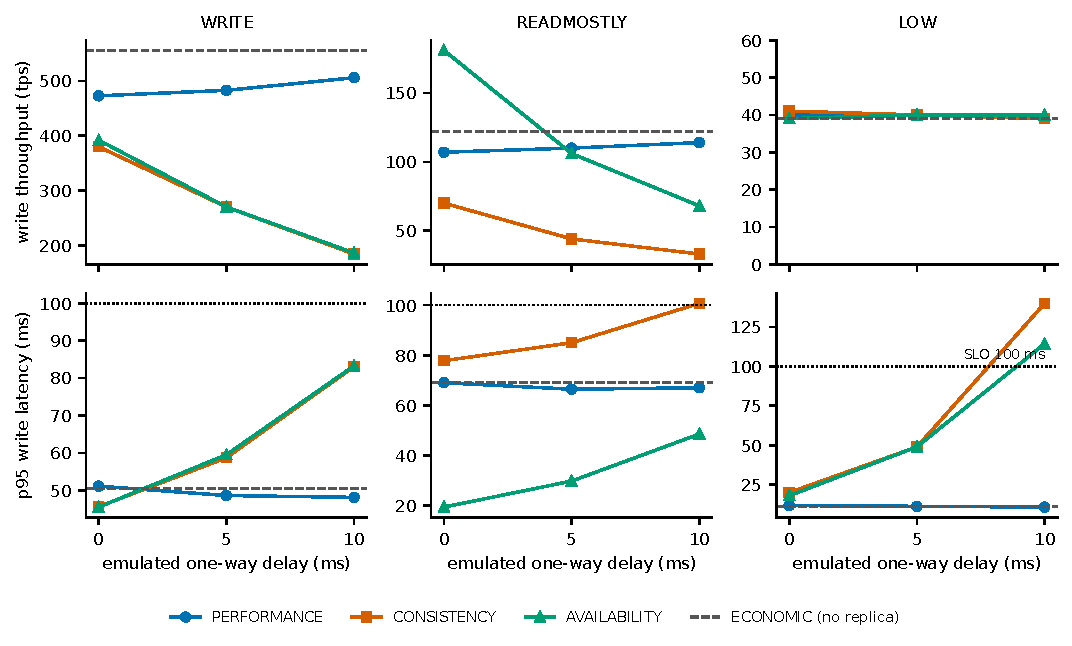
\includegraphics[width=\textwidth]{figures/fig_grid.pdf}
\caption{Write throughput (top) and p95 write latency (bottom) by mode, workload and emulated one-way delay (means over five repetitions). The dotted line is the 100\,ms bound; the dashed line is \econ, measured at 0\,ms only.}\label{fig:grid}
\end{figure}

\begin{table}[t]
\centering\small
\resizebox{\textwidth}{!}{\begin{tabular}{llccc}
\toprule
Mode & Workload & CPU of primary, \% of limit [range over delays] & Memory, \% of limit & Active connections \\
\midrule
\textsc{performance} & \textsc{write} & 99 (99--100) & 99 & 6.2 \\
\textsc{performance} & \textsc{readmostly} & 100 (100--100) & 98 & 3.2 \\
\textsc{performance} & \textsc{low} & 15 (15--15) & 97 & 1.1 \\
\addlinespace
\textsc{consistency} & \textsc{write} & 71 (49--95) & 99 & 8.0 \\
\textsc{consistency} & \textsc{readmostly} & 100 (100--100) & 99 & 3.9 \\
\textsc{consistency} & \textsc{low} & 18 (17--19) & 99 & 1.6 \\
\addlinespace
\textsc{availability} & \textsc{write} & 72 (50--96) & 99 & 8.0 \\
\textsc{availability} & \textsc{readmostly} & 36 (21--56) & 99 & 2.7 \\
\textsc{availability} & \textsc{low} & 14 (14--15) & 99 & 1.7 \\
\addlinespace
\textsc{economic} & \textsc{write} & 100 & 99 & 5.8 \\
\textsc{economic} & \textsc{readmostly} & 100 & 99 & 3.2 \\
\textsc{economic} & \textsc{low} & 13 & 99 & 1.1 \\
\bottomrule
\end{tabular}}
\caption{Telemetry of the primary during the grid (means over repetitions; CPU as a percentage of the one-CPU limit).}
\label{tab:telemetry}
\end{table}
\noindent Table~\ref{tab:telemetry} summarises the telemetry collected on the primary.

\subsection{Dependence on client concurrency (RQ1)}\label{sec:sweep}
The grid uses eight clients, so its throughput price of synchrony applies to that concurrency only. Table~\ref{tab:sweep} and Figure~\ref{fig:sweep} give the sweep. Measured mean latency agrees with $N/\mathrm{tps}$ within 0.7\% in every run, which supports the closed-loop reading. With eight clients the sweep reproduces the grid within about 10\% (\cons\ 368, 253 and 170\,tps at 0, 5 and 10\,ms against 380, 270 and 184; \perf\ 509--527 against 473--506\,tps).

A control with four pgbench threads instead of two at 32 clients (0 and 10\,ms, both modes, five repetitions) gave throughput within 9\% of the two-thread runs in every cell (ratios 0.91--1.01); the largest difference was a lower value for \cons\ at 10\,ms (242 against 266\,tps, about two standard errors). The number of load-generator threads therefore does not explain the plateau of \perf\ at about 480--530\,tps, although the generator still shares the host with the database.

Two regimes appear. With two clients the primary is not saturated (CPU 76\% under \perf) and the extra latency of \cons\ is one round trip: $k=0.99$ [0.94, 1.03]. The throughput loss is then the largest, 41\%, 71\% and 81\% at 0, 5 and 10\,ms. With eight and 32 clients \perf\ saturates the one-CPU primary (99--100\% CPU, about 480--530\,tps regardless of delay) and the loss shrinks to 19--45\% at 32 clients, but does not vanish: at 10\,ms \cons\ still delivers 45\% less than \perf. In this regime the extra latency exceeds one round trip ($k=1.32$ [1.13, 1.65] with eight and $1.87$ [1.54, 2.19] with 32 clients). We did not test why; longer-held row locks while a commit waits for the standby are one candidate, since scale factor 10 gives only ten branch rows, but this is a hypothesis. The model with $L_0$ fixed at its eight-client value does not transfer: it underestimates throughput at two clients (observed over predicted 1.6--2.1) and overestimates it at 32 (0.25--0.39), which is consistent with queueing at a saturated primary. What transfers is the order of magnitude of the latency cost, not a single formula. The first repetition was lower than the others in some synchronous cells (for example 293 against 362--405\,tps at eight clients and 0\,ms), possibly a cold-start effect; excluding it changes the throughput losses by at most about three points and $k$ to 1.01, 1.17 and 2.01 for 2, 8 and 32 clients.

\begin{table}[t]
\centering\small
\resizebox{\textwidth}{!}{\begin{tabular}{rcccccc}
\toprule
& \multicolumn{3}{c}{Throughput loss of \cons\ vs \perf, \% [95\% CI]} & & & \\
\cmidrule(lr){2-4}
Clients & 0\,ms & 5\,ms & 10\,ms & $k$ [95\% CI] & $L_0$ (ms) & \perf\ CPU (\%) \\
\midrule
2 & 41 [36, 47] & 71 [70, 73] & 81 [81, 82] & 0.99 [0.94, 1.03] & 9.7 & 76 \\
8 & 28 [23, 35] & 50 [48, 52] & 68 [65, 72] & 1.32 [1.13, 1.65] & 20.8 & 99 \\
32 & 19 [16, 25] & 29 [26, 31] & 45 [44, 48] & 1.87 [1.54, 2.19] & 79.9 & 100 \\
\bottomrule
\end{tabular}
}
\caption{Client-count sweep (write workload, five repetitions): throughput loss of \cons\ relative to \perf\ at each one-way delay, with percentile bootstrap 95\% intervals over repetitions; slope $k$ and intercept $L_0$ of the fit $L=L_0+k\cdot\mathrm{RTT}$ for \cons; mean CPU of the primary under \perf.}\label{tab:sweep}
\end{table}
\begin{figure}[t]
\centering
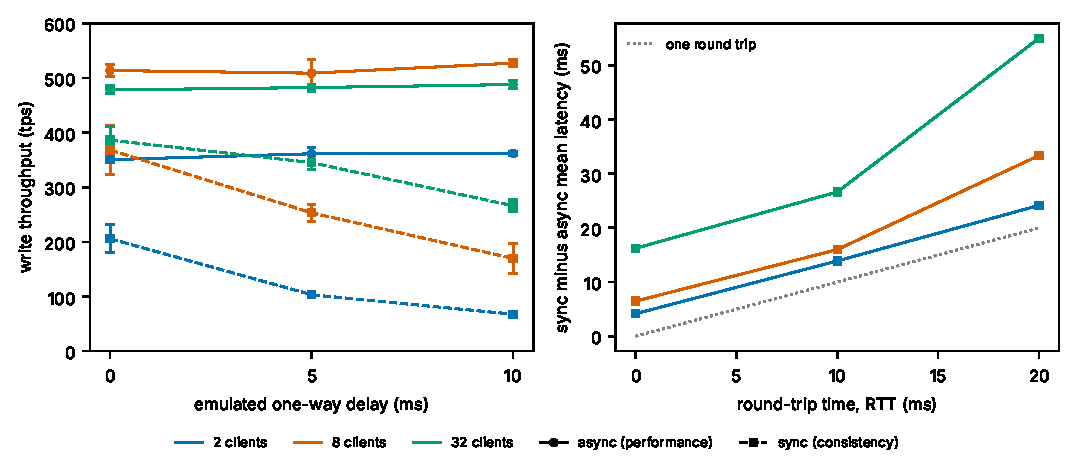
\includegraphics[width=\textwidth]{figures/fig_sweep.pdf}
\caption{Left: write throughput (mean $\pm$ s.d. over five repetitions) by delay, client count and mode. Right: mean latency of \cons\ minus that of \perf\ against round-trip time; the dotted line is one round trip.}\label{fig:sweep}
\end{figure}

\subsection{Protection (RQ2)}
\begin{table}[t]
\centering\small
\resizebox{\textwidth}{!}{\begin{tabular}{lrrrrrrr}
\toprule
Level & Isol.\ (s) & Runs & Runs with loss & Lost, mean [95\% CI] & Lost per s & Writes resume (s) & Promotion (s) \\
\midrule
ASYNC & 1 & 3 & 3/3 & 2053 [1881, 2262] & 2053 & 6.3 [6.2--9.1] & 5.9 \\
ASYNC & 2 & 6 & 6/6 & 4074 [3676, 4470] & 2037 & 5.2 [3.8--7.4] & 3.3 \\
ASYNC & 5 & 3 & 3/3 & 10842 [10539, 11008] & 2168 & 3.2 [3.1--3.4] & 2.7 \\
SYNC\_1 & 1 & 3 & 0/3 & 0 & 0 & 13.6 [9.0--14.1] & 5.6 \\
SYNC\_1 & 2 & 6 & 0/6 & 0 & 0 & 11.8 [5.2--28.1] & 4.5 \\
SYNC\_1 & 5 & 3 & 0/3 & 0 & 0 & 10.9 [10.7--12.4] & 3.9 \\
SYNC\_2 & 2 & 6 & 0/6 & 0 & 0 & 12.4 [9.1--31.7] & 4.4 \\
\bottomrule
\end{tabular}
}
\caption{Isolation-then-crash results at 5\,ms delay. Lost = acknowledged transactions absent from the new primary. Writes resume = median [min--max] seconds from the crash to the first successful write; promotion = median seconds to a new primary.}\label{tab:rpo}
\end{table}

\begin{figure}[t]
\centering
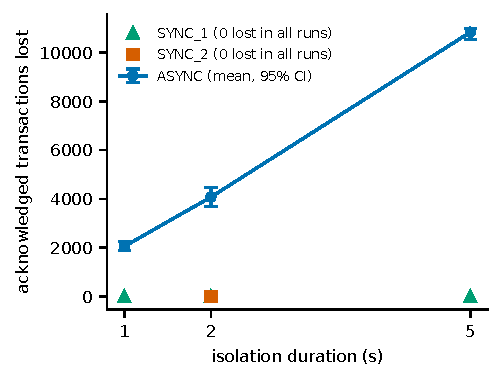
\includegraphics[width=0.55\textwidth]{figures/fig_loss.pdf}
\caption{Acknowledged transactions lost versus isolation duration. Asynchronous: mean and bootstrap 95\% interval; synchronous: zero in every run.}\label{fig:loss}
\end{figure}

Asynchronous replication lost acknowledged transactions in all 12 runs (Wilson lower bound 76\%), and the loss grew with the isolation: 2,053, 4,074 and 10,842 transactions on average for 1, 2 and 5\,s, that is 2,053, 2,037 and 2,168 per second (Table~\ref{tab:rpo}, Figure~\ref{fig:loss}). The loss per second of isolation is therefore roughly constant, so the loss is proportional to the duration; its absolute value depends on the write rate of our load and on how long the isolated primary keeps acknowledging writes; we vary the write rate below. Synchronous replication lost no acknowledged transaction in 18 of 18 runs (12 with one synchronous replica, 6 with two; Wilson upper bound for the proportion of runs with loss: 17.6\%), because commits stop being acknowledged when no standby confirms them.

Promotion was fast in all configurations (medians 2.7--5.9\,s). Writes resumed later with synchronous replication (medians 10.9--13.6\,s, \textsc{sync\_2} 12.4\,s) than with asynchronous replication (3.2--6.3\,s). We did not measure the cause; a plausible one is that the new primary has to re-establish its synchronous standby before acknowledging commits. The former primary was re-cloned by our script in 25 of 30 runs, because it did not rejoin within four minutes, which reflects the instability of our testbed more than a property of the modes.

\paragraph{Loss and write rate.} Table~\ref{tab:rate} gives the rate-limited runs. The loss grew with the rate: 566, 1,128 and 2,456 transactions on average at 250, 500 and 1,000\,tps, that is 1.13, 1.13 and 1.23 times the product of rate and the nominal 2\,s. A linear fit over the 12 runs gives an intercept of $-99$ transactions and a slope of 1.27 against that product, so the loss is roughly proportional to the write rate. The excess over rate $\times$ time (13--23\%) is systematic and we did not explain it; candidates are an isolation window longer than the nominal one, since the container is stopped and the network restored after the wait, and replication lag present before the isolation. The unthrottled runs above cannot be placed on this line because we did not record their write rate during the isolation. The runs have four repetitions per rate, so we give ranges rather than intervals.

\paragraph{Crash without isolation.} Killing the primary without isolating it lost no acknowledged transaction in 10 of 10 runs (five \textsc{async}, five \textsc{sync\_1}; Wilson upper bound for the proportion of runs with loss: 28\% overall, 43\% per mode) and left no unacknowledged row (Table~\ref{tab:crash}). In our setup the loss under asynchrony therefore required the primary to keep acknowledging writes while cut off from its standbys; the crash alone did not produce it. The time to a new primary in this scenario was 102.7--103.9\,s in all ten runs, and writes resumed after 103.2--109.5\,s, against 2.5--7.8\,s after an isolation. Such a stable value points to a fixed delay rather than a property of the replication mode; we did not identify it. The two scenarios also differ in how the primary is stopped (container stopped, then pod deleted, versus pod deleted only), and this series ran on the rebuilt testbed. We therefore do not compare recovery times across the two scenarios.

\paragraph{Unacknowledged rows.} Synchronous replication lost no acknowledged transaction, but 8 of 18 synchronous isolation runs left rows on the new primary that no client had seen acknowledged: 46 rows in total (13 and 12 with one synchronous replica at $T=1$ and 2\,s, none at 5\,s; 21 with two at 2\,s), at most seven in a run, which is within one in-flight transaction per client (eight clients). A plausible reading is that these transactions were committed and streamed before the acknowledgement reached the client or before the primary stopped; we did not test it. A client that retries a request it never saw acknowledged may therefore duplicate it after a failover. The asynchronous runs had none.

\begin{table}[t]
\centering\small
\resizebox{0.85\textwidth}{!}{\begin{tabular}{rrrrrr}
\toprule
Rate limit (tps) & Runs & Lost (mean) & Lost (min--max) & Rate $\times$ 2\,s & Lost / (rate $\times$ 2\,s) \\
\midrule
250 & 4 & 566 & 537--587 & 500 & 1.13 \\
500 & 4 & 1128 & 1092--1154 & 1000 & 1.13 \\
1000 & 4 & 2456 & 2175--2823 & 2000 & 1.23 \\
\bottomrule
\end{tabular}
}
\caption{Asynchronous replication, isolation of 2\,s at 5\,ms delay, with the write rate of the eight clients limited by pgbench. Lost = acknowledged transactions absent from the new primary.}\label{tab:rate}
\end{table}
\begin{table}[t]
\centering\small
\resizebox{\textwidth}{!}{\begin{tabular}{llrrrrrr}
\toprule
Scenario & Level & Runs & With loss & Lost (mean) & Unacknowl.\ rows & Promotion (s) & Writes resume (s) \\
\midrule
crash only & \textsc{async} & 5 & 0 & 0 & 0 (0 runs) & 102.7--103.9 & 103.2--105.8 \\
crash only & \textsc{sync\_1} & 5 & 0 & 0 & 0 (0 runs) & 102.9--103.5 & 104.5--109.5 \\
isolation 1\,s & \textsc{async} & 3 & 3 & 2053 & 0 (0 runs) & 5.4--6.6 & 6.2--9.1 \\
isolation 1\,s & \textsc{sync\_1} & 3 & 0 & 0 & 13 (2 runs) & 2.6--6.5 & 9.0--14.1 \\
isolation 2\,s & \textsc{async} & 6 & 6 & 4074 & 0 (0 runs) & 2.5--4.6 & 3.8--7.4 \\
isolation 2\,s & \textsc{sync\_1} & 6 & 0 & 0 & 12 (2 runs) & 3.2--6.3 & 5.2--28.1 \\
isolation 2\,s & \textsc{sync\_2} & 6 & 0 & 0 & 21 (4 runs) & 2.7--7.8 & 9.1--31.7 \\
isolation 5\,s & \textsc{async} & 3 & 3 & 10842 & 0 (0 runs) & 2.6--2.8 & 3.1--3.4 \\
isolation 5\,s & \textsc{sync\_1} & 3 & 0 & 0 & 0 (0 runs) & 3.9--5.7 & 10.7--12.4 \\
\bottomrule
\end{tabular}
}
\caption{All protection runs at 5\,ms delay, including the crash-only scenario and the count of unacknowledged rows present on the new primary (sum over runs, with the number of runs concerned). Promotion and writes resume are ranges (min--max) of seconds from the stop of the primary.}\label{tab:crash}
\end{table}

\subsection{Measured best mode per context (RQ3)}
\begin{table}[t]
\centering\small
\begin{tabular}{llll}
\toprule
Workload & Requirements & Label (0, 5, 10\,ms) & Bootstrap confidence \\
\midrule
\textsc{low} & none & \econ, \econ, \econ & 100\%, 100\%, 100\% \\
\textsc{readmostly} & HA & \perf, \perf, \perf & 100\%, 100\%, 100\% \\
\textsc{write} & durable, HA & \cons, \cons, \cons & 96\%, 99\%, 100\% \\
\bottomrule
\end{tabular}
\caption{Labels under the \textsc{balanced} policy with a 100\,ms p95 write bound. Confidence is the share of bootstrap resamples (over repetitions) giving the same label.}\label{tab:labels}
\end{table}

Under \textsc{balanced}, the label is \econ\ for \textsc{low}, \perf\ for \textsc{readmostly} and \cons\ for \textsc{write}, at every delay (Table~\ref{tab:labels}); \avail\ appeared as the label only in 4\% and 1\% of bootstrap resamples for \textsc{write} at 0 and 5\,ms. The labels are stable under measurement noise but depend mostly on the declared requirements: with the 100\,ms bound the measurements decide only ties and feasibility. Sensitivity to the parameters is as follows (share of the nine contexts whose label is unchanged). Bound $L$ = 50, 75, 100, 150, 200\,ms: 67, 100, 100, 100, 100\%. Throughput weight 0, 0.1, 1: 100\% each. Tie tolerance 0, 2, 5, 10\%: 67, 89, 100, 100\%. Policy \textsc{default}, \textsc{balanced}, \textsc{strict}: 67, 100, 33\%. The policy dominates.

Measurements also reveal a context without feasible mode. Under \textsc{strict}, \textsc{low} at 10\,ms has no durable mode within the bound (p95 write latency 114\,ms at best), so the oracle itself violates the latency bound in one of nine contexts (11.3\% of replayed steps, Table~\ref{tab:replay}). A controller should signal such a context rather than choose silently.

\subsection{Rule cascade versus measured labels (RQ3, RQ4)}
Applied to the 150 measured cells, the cascade of our earlier papers agrees with the measured label (\textsc{balanced}) in 68.7\% of cells (Cohen's $\kappa=0.53$). It predicts \cons\ for 40 of the 50 \textsc{readmostly} cells whose label is \perf, and \perf\ for 7 of the 50 \textsc{write} cells whose label is \cons, where durability is required; it matches the \econ\ label in all 50 \textsc{low} cells, which follows from our declared off-peak hour for \textsc{low} rather than from an independent signal. Agreement is 82\% when the telemetry was measured under \avail, 58\% under \cons, 67\% under \perf\ and 67\% under \econ, so the cascade's output depends on the mode that produced its inputs.

Recalibrating the cascade does not close the gap in the grid we searched. Over 36 settings (throughput thresholds scaled by 1, 0.5, 0.25 or 0.1; CPU thresholds 85/95/none and 50/70/90\%), the published thresholds already give the highest agreement (68.7\%, $\kappa=0.53$, 11.3\% of cells violating a constraint); the lowest violation rate, 6.7\%, comes with throughput thresholds divided by four and an agreement of 50\% ($\kappa=0.25$). The best setting is chosen on the same data and is therefore optimistic. Over the whole grid, the replication lag measured on the primary never exceeded 0.10\,MB (threshold of the cascade: 100\,MB), the rollback rate never exceeded 0.00\% of transactions (threshold: 1\%), and 0 deadlocks were recorded (threshold: 5 per window). The first branch of the cascade therefore never fires on this testbed.


\subsection{Replay of controllers (RQ4)}
\begin{table}[t]
\centering\small
\resizebox{\textwidth}{!}{\begin{tabular}{lccccc}
\toprule
Controller & \multicolumn{3}{c}{Steps in violation, \% [95\% CI over traces]} & Cost & Switches \\
\cmidrule(lr){2-4}
 & \textsc{balanced} & \textsc{default} & \textsc{strict} & (\textsc{bal.}) & (\textsc{bal.}) \\
\midrule
Fixed \textsc{performance} & 34.7 [32.2, 37.2] & 66.6 [64.1, 69.0] & 100.0 [100.0, 100.0] & 2.00 & 0.0 \\
Fixed \textsc{consistency} & 19.8 [17.0, 22.7] & 19.8 [17.0, 22.7] & 19.8 [17.0, 22.7] & 3.00 & 0.0 \\
Fixed \textsc{availability} & 11.3 [9.4, 13.3] & 11.3 [9.4, 13.3] & 11.3 [9.4, 13.3] & 3.00 & 0.0 \\
Fixed \textsc{economic} & 66.6 [64.2, 69.0] & 66.6 [64.2, 69.0] & 100.0 [100.0, 100.0] & 1.00 & 0.0 \\
\midrule
Rule cascade [earlier papers] & 13.2 [11.3, 15.1] & 13.2 [11.3, 15.1] & 46.6 [43.9, 49.4] & 2.28 & 6.2 \\
Random forest (measured labels) & 0.0 [0.0, 0.0] & 0.4 [0.2, 0.5] & 11.3 [9.3, 13.3] & 2.02 & 5.2 \\
Oracle (measured labels) & 0.0 [0.0, 0.0] & 0.0 [0.0, 0.0] & 11.3 [9.3, 13.3] & 2.01 & 5.2 \\
\bottomrule
\end{tabular}
}
\caption{Replay of 300 random traces of 24 steps: share of steps violating durability, HA or the 100\,ms latency bound under each declared policy (percentile bootstrap intervals over traces). Cost and switches are given for the \textsc{balanced} policy.}\label{tab:replay}
\end{table}

\begin{figure}[t]
\centering
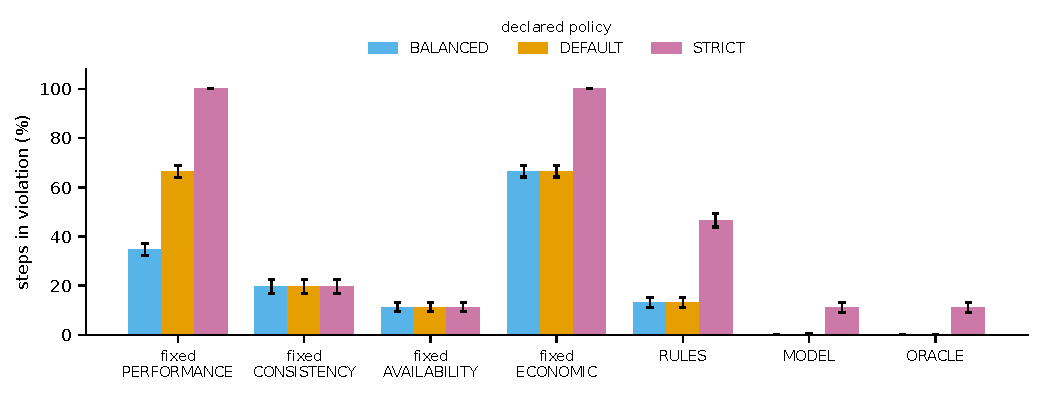
\includegraphics[width=\textwidth]{figures/fig_replay.pdf}
\caption{Steps in violation by controller and declared policy, with 95\% intervals over traces.}\label{fig:replay}
\end{figure}

No fixed mode is acceptable in all contexts (Table~\ref{tab:replay}, Figure~\ref{fig:replay}): the best, \avail, violates the latency bound in 11.3\% of steps, \cons\ in 19.8\%, and \perf\ and \econ\ violate the durability or HA requirements in 35--100\% of steps depending on the policy. The rule cascade violates the requirements in 13.2\% of steps under \textsc{balanced} and \textsc{default} (5\% durability, 8\% latency) and in 46.6\% under \textsc{strict} (38\% durability, 33\% HA, 8\% latency), at a mean cost of 2.28 instances against 2.01 for the oracle under \textsc{balanced}. The two figures coincide because the decisions of the cascade do not depend on the policy and, in the replay, it chose \cons\ at every \textsc{readmostly} step, so that under both policies only the \textsc{write} steps, where it sometimes chose \perf, violate durability. The random forest trained on measured labels matches the oracle (0.0, 0.4 and 11.3\% of steps in violation; the oracle's 11.3\% under \textsc{strict} comes from the infeasible context). This result is expected rather than informative on its own: the telemetry separates the three workload types easily and the label is a function of workload and policy, so the forest recovers the policy it is trained with. In leave-one-delay-out evaluation the forest reached 0.967 accuracy and 0.967 macro-F1 against 0.687 and 0.648 for the cascade, but the delay never changes the label, so this test is not demanding.

\section{Discussion}\label{sec:discussion}
\paragraph{Requirements must be inputs}
The cascade of our earlier work encodes one implicit requirement set, which resembles our \textsc{balanced} and \textsc{default} policies; when requirements tighten, its violations rise from 13\% to 47\% of steps. A controller that receives the requirements and the measured cost of each mode reaches the oracle in our replay, and can also report that no mode is feasible. The contribution of measurement is not a better classifier but numbers that the requirements can be checked against: a throughput price for synchrony that grew from about 20\% to 64\% of write throughput as the delay went from 0 to 10\,ms with eight clients (19--81\% across 2 to 32 clients and the three delays), a latency price of about one round trip per commit when the primary is not saturated, and a loss of about 2,000 acknowledged transactions for each second of isolation under asynchrony.

\paragraph{The cost of synchrony depends on the load}
The same delay costs 81\%, 68\% or 45\% of write throughput at 10\,ms depending on whether two, eight or 32 clients drive the primary. A controller that reacts to the inter-node delay alone would misjudge the price of synchrony; the load that the primary carries has to be an input as well. This also qualifies our grid numbers, which come from one concurrency level and a baseline (\perf) that already saturates the CPU of the primary.

\paragraph{Implications for practice}
On this testbed, in the isolation scenario, one and two synchronous standbys gave the same protection (no loss), and the throughput price of synchrony grew with inter-node delay; at 10\,ms and a 100\,ms bound, no durable mode served a lightly loaded workload. A practitioner should therefore estimate the delay between nodes and the isolation durations they are willing to tolerate before choosing a mode, rather than rely on thresholds on CPU or throughput. These figures depend on the testbed and should not be transferred to other deployments.

\paragraph{Role of \avail}
Under none of our policies is \avail\ the selected mode, and it is indistinguishable from \cons\ for writes. Its read benefit at 0\,ms is real in our data but confounded with its extra instance and, at larger delays, with client placement. We therefore do not present it as a finding.

\section{Threats to validity}\label{sec:threats}
\emph{Construct.} Requirements and the 100\,ms bound are declared; the labels follow from them. The mapping of modes to operator parameters and the \textsc{low}-as-off-peak mapping are ours. Telemetry is observed under the mode in operation, which affects the rule cascade.
\emph{Internal.} We used CloudNativePG v1.22.0; we did not test whether more recent operator versions, which may fence an isolated primary, change the loss we report. One host runs three worker nodes, the primary, standbys and load generator, so they share CPU, memory and storage; the delay is emulated and applies to egress only. Pod CPU limits make several cells CPU-bound, and the memory of the primary reported by the container cgroup sits at 97--99\% of its limit in every cell; we did not separate file cache from resident memory. We observed instability (re-cloned replicas in 25 of 30 protection runs, a replica not streaming before some runs) and mitigated it with explicit pre-run checks and re-cloning, which may affect recovery times. Table bloat reduced throughput in an earlier run; the final runs reset and vacuum the tables.
\emph{External.} One database, one operator, one host, three synthetic workloads and nine contexts; no production traces. The loss figure depends on the write rate and on the isolation durations we chose; the rate-limited test has four runs per rate and an unexplained excess of 13--23\% over rate $\times$ time, and the crash-only runs ran on a rebuilt testbed and show a 103\,s time to a new primary that we did not explain. The client sweep uses one transaction type, one scale factor, three client counts and three delays; its load generator shares the host with the database and may compete for CPU; a control with four instead of two pgbench threads at 32 clients did not change throughput, which excludes the thread count but not this competition.
\emph{Conclusion.} Few repetitions per protection cell (3--6); the fits of the synchronous latency model have one degree of freedom, and the explanation of $k>1$ under saturation is untested; one run of the sweep was discarded after a host suspension and re-run in full; intervals over replayed traces describe trace sampling only; the oracle and violation metrics depend on the same declared policy; transition costs and a closed-loop controller were not evaluated.

\section{Conclusion}\label{sec:conclusion}
We measured what four replication modes cost and protect on containerised PostgreSQL, derived the best mode per context from measurements under declared requirements, and replayed controllers on the measured outcomes. Asynchronous replication lost about 2,000 acknowledged transactions per second of isolation while synchronous replication lost none (though 8 of 18 synchronous runs left some unacknowledged rows on the new primary), and a crash without isolation lost nothing in either mode; the loss scaled with the write rate. The synchronous price was a latency price of about one network round trip per commit when the primary is not saturated, which translated into a throughput price that grew with inter-node delay and shrank, without vanishing, as client concurrency saturated the primary. No fixed mode met the requirements everywhere, a static rule cascade violated them in 13--47\% of steps, and one context had no feasible durable mode. Future work should evaluate a closed-loop controller on a multi-host cluster with real network delay, measure the cost of mode transitions, test readers placed on standbys, and use production traces.

\section*{Availability of data and code}\label{sec:avail}
Scripts, raw measurements and analysis code are available at \url{\repourl} (code under the MIT licence, data under CC BY 4.0), with an archived release on Zenodo.

\section*{Declaration of competing interest}
The authors declare that they have no known competing financial interests or personal relationships that could have appeared to influence the work reported in this paper.

\section*{Funding}
The authors did not receive support from any organisation for the submitted work.

\section*{Declaration of generative AI and AI-assisted technologies in the writing process}
During the preparation of this work the authors used an AI assistant (Claude, Anthropic) to help develop measurement and analysis scripts, to assist with the analysis of the results and to draft and edit text. The authors ran all experiments, reviewed and edited all content, and take full responsibility for the content of the publication.

\bibliographystyle{elsarticle-num}
\bibliography{refs}
\end{document}
